\chapter{Giới thiệu}
\label{chap:chap1-introduce}
\section{Khái quát chung}

Trong kỷ nguyên mà sự phát triển của các hệ thống điện toán đám mây càng phát
triển với độ nở lớn như hiện nay, lượng dữ liệu đổ lên các dịch vụ đám mây đang tăng
theo cấp số nhân. Đại dịch Covid-19 vẫn đang lan rộng, thành tựu về vắc – xin tuy đã
kiểm soát khá tốt tốc độ lây lan của dịch bệnh, nhưng vẫn chưa thể xóa sổ hoàn toàn nó
ra khỏi đời sống kinh tế, xã hội. Dịch bệnh thúc đẩy phát triển những cách làm việc phi
truyền thống, chuyển dần sang nền tảng trực tuyến, nơi mà dòng chảy dữ liệu vốn đã
chật chội nay càng thêm khó kiểm soát. Vào năm 2020, tổng chi tiêu của người dùng
cuối cho các dịch vụ đám mây đạt tổng cộng 270 tỷ USD, con số này dự kiến sẽ tăng với
mức đáng kinh ngạc là 23,1\% vào năm 2021, lên 332,3 tỷ USD. Trong khi đó, 48\%
doanh nghiệp chọn lưu trữ dữ liệu quan trọng của họ, bao gồm dữ liệu mã hóa và dữ liệu
thông thường trên đám mây. Vì vậy, không có gì ngạc nhiên khi 75\% doanh nghiệp coi
các vấn đề bảo mật đám mây là mối quan tâm hàng đầu. Trong số đó, 33\% người được
hỏi cực kỳ quan tâm, 42\% cực kỳ lo ngại và 25\% không quan tâm hoặc quan tâm vừa
phải \cite{vladimir2021cloudcomputing}. \\
\indent Vì nhiều công nghệ điện toán đám mây đang ngày càng được sử dụng nhiều hơn,
và do đó, giống như hầu hết các công nghệ mới, vấn đề bảo mật cho nó đã, đang và tiếp
tục được đặt ra và ngày càng trở nên quan trọng. Dữ liệu là nguồn sống của doanh nghiệp,
và khi nó càng lớn thì động lực bảo vệ tài sản quý giá này thúc đẩy họ tìm kiếm các giải
pháp bảo mật an toàn hơn. Vấn đề chính đặt ra là tìm một nhà cung cấp dịch vụ đám mây
(CSP) có uy tín và ổn định để các doanh nghiệp có thể ít bị tấn công hơn hay bản thân
các công ty phải chủ động phát triển một công cụ như là chìa khóa két sắt để bảo vệ tài
sản của mình khi giao cho người khác nắm giữ. \\
\indent Cả hai hướng tiếp cận này đều có những ưu và nhược điểm. Sử dụng dịch vụ của
một đối tác CSP uy tín giúp chủ sở hữu dữ liệu tiết kiệm được nhiều kinh phí, mức độ
tin cậy cũng được đảm bảo ở mức tương đối. Tuy nhiên, hướng tiếp cận này chỉ giải quyết được một số vấn đề xảy ra từ những đối tượng xấu có ý đồ tấn công mà không giải
quyết được các vấn đề có thể xảy ra từ bên cung cấp dịch vụ. Ngược lại, để phát triển
một giải pháp bảo mật hiệu quả, nguồn lực kinh phí và con người phải bỏ ra là rất lớn.
Không phải công ty, doanh nghiệp nào cũng có thể đầu tư nguồn lực lớn vào vấn đề này. \\
\indent Nhằm khắc phục điểm yếu và phát huy điểm mạnh của hai hướng trên, việc một
bên thứ ba có đầy đủ năng lực chuyên môn và nguồn lực tài chính đứng ra phát triển dịch
vụ bảo mật trên nền tảng đám mây giải quyết được cả hai vấn đề nếu trên: dịch vụ cung
cấp cho mỗi doanh nghiệp sử dụng nên giá dịch vụ sẽ rẻ hơn so với tự phát triển; bên thứ
ba được đảm bảo và chứng nhận độc lập với CSP hoàn toàn đã tránh được các rủi ro chủ
quan phát sinh. Nói tóm lại, sự xuất hiện và phát triển của một bên thứ ba đảm nhiệm
vai trò bảo mật cơ sở dữ liệu trên dịch vụ đám mây xuất phát từ nhu cầu thực tế của các
bên liên quan, hứa hẹn sẽ mang đến những tiện ích và trải nghiệm tuyệt vời cho người
dùng, nhất là các doanh nghiệp và là hướng đi tiềm năng phát triển trong tương lai. \\
\section{Báo cáo vấn đề}
Trước sự phát triển mạnh mẽ của các dịch vụ lưu trữ đám mây, nguy cơ tấn công
vào các cơ sở dữ liệu này đang tiềm ẩn trên hầu hết khu vực và đa dạng các đối tượng
nạn nhân, kể cả các công ty lớn chuyên cung cấp dịch vụ lưu trữ đám mây như Google
Cloud hay AWS. \\
\indent McAfee đã tiến hành một nghiên cứu về các cuộc tấn công mạc vào các dịch vụ
đám mây để xác định xem liệu có sự gia tăng các cuộc tấn công kể từ khi đại dịch Covid19 bắt đầu hay không. Kết quả cho thấy sự gia tăng lên đến 630\% các cuộc tấn công
mạng vào các dịch vụ đám mây kể từ tháng 1 đến tháng 4 năm 2020. Với sự mở rộng
của các dịch vụ chăm sóc sức khỏe qua điện thoại, nhiều nhà cung cấp dịch vụ đã chuyển
sang sử dụng dịch vụ đám mây. Trong quý đầu tiên năm 2020, đây là ngành bị nhắm
mục tiêu đa số trong các cuộc tấn công với khoảng 198 triệu IP độc hại được phát hiện \cite{mcafee2020risk}.
\begin{figure}
    \centering
    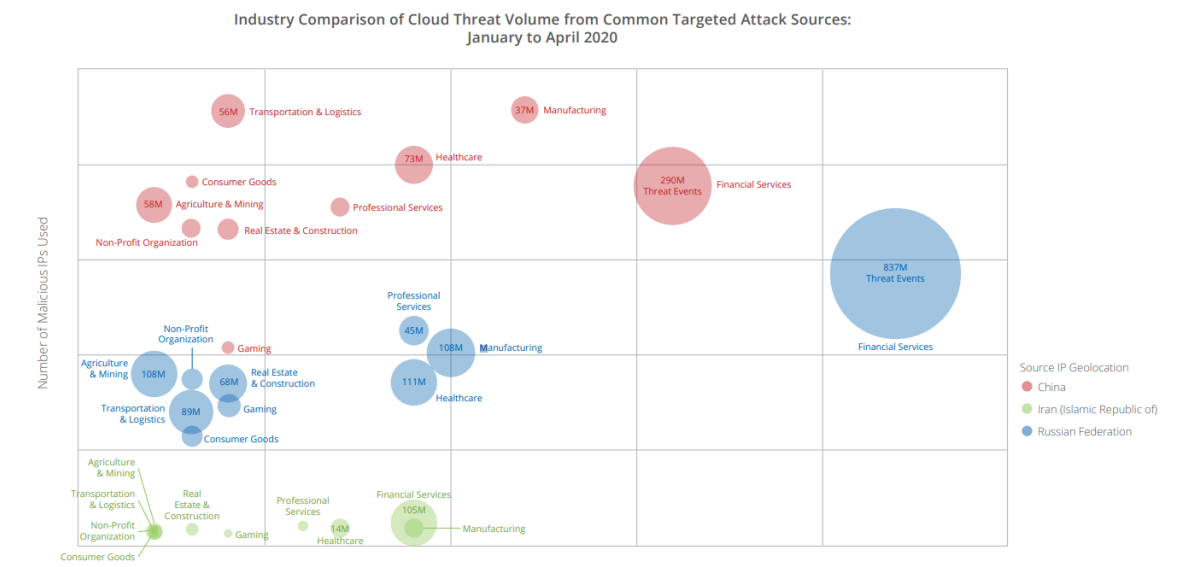
\includegraphics[scale=0.5]{graphics/chapter-1/chap1-mcafee.png}
    \caption{Số tổ chức bị tấn công \cite{mcafee2020risk}}
    \label{fig:chap1-mcafee}
\end{figure}
\section{Cơ sở lý thuyết và phương pháp luận}
Trong khóa luận này, nhóm tác giả sử dụng kỹ thuật kiểm soát truy cập dựa trên
thuộc tính, thông qua các phiên bản ứng dụng của mã hóa dựa trên thuộc tính. Đây là kỹ
thuật được phát triển thêm từ kiểm soát truy cập dựa trên vai trò. Kiểm soát truy cập dựa
trên thuộc tính không phân chia vai trò cho từng người dùng mà cấp quyền truy cập cho
họ thông qua một tập thuộc tính biểu thị chính sách truy cập. Người dùng có những thuộc
tính thỏa mãn chính sách được quy định có thể đọc được tài liệu mã hóa. \\
\indent Bên cạnh đó tìm hiểu, nghiên cứu một số phương pháp thao tác trên cơ sở dữ liệu
mã hóa để đảm bảo quyền riêng tư dữ liệu của người dùng trước các máy chủ đám mây
bên thứ ba không đáng tin cậy.
\section{Đối tượng và phạm vi thực hiện}
\subsection{Đối tượng nghiên cứu}
\begin{itemize}
    \item Kỹ thuật kiểm soát truy cập dựa trên thuộc tính, kỹ thuật mã hóa dựa trên thuộc tính, phương pháp mã hóa chính sách khóa dựa trên thuộc tính, phương pháp mã hóa chính sách bản mã dựa trên thuộc tính.
    \item Mã hóa đồng cấu, lược đồ searchable encryption.
    \item Hệ quản trị cơ sở dữ liệu quan hệ có cấu trúc SQL.
\end{itemize}
\subsection{Phạm vi thực hiện}
Phân tích và đánh giá mô hình kiểm soát truy cập dựa trên thuộc tính trên dữ liệu mã hóa; hỗ trợ các thao tác tìm kiếm, cập nhật trên dữ liệu mã hóa; kết hợp triển khai trên hệ quản trị cơ sở dữ liệu MySQL.
\subsection{Mục tiêu nghiên cứu}
Tìm hiểu về các kỹ thuật, phương pháp, thuật toán nhằm kiểm soát truy cập dựa trên thuộc tính; hỗ trợ các thao tác trên dữ liệu mã hóa; từ đó xây dựng một ứng dụng nhằm đánh giá mức độ hiệu quả của phương pháp đối với khả năng bảo mật dữ liệu trên dịch vụ đám mây.
